\documentclass[12pt,a4paper]{article}%
%Options -- Point size:  10pt (default), 11pt, 12pt
%        -- Paper size:  letterpaper (default), a4paper, a5paper, b5paper
%                        legalpaper, executivepaper
%        -- Orientation  (portrait is the default)
%                        landscape
%        -- Print size:  oneside (default), twoside
%        -- Quality      final(default), draft
%        -- Title page   notitlepage, titlepage(default)
%        -- Columns      onecolumn(default), twocolumn
%        -- Equation numbering (equation numbers on the right is the default)
%                        leqno
%        -- Displayed equations (centered is the default)
%                        fleqn (equations start at the same distance from the right side)
%        -- Open bibliography style (closed is the default)
%                        openbib
% For instance the command
%           \documentclass[a4paper,12pt,leqno]{article}
% ensures that the paper size is a4, the fonts are typeset at the size 12p
% and the equation numbers are on the left side

% Tabelas
\usepackage{multirow}

% Símbolos Matemáticos
\usepackage{amsmath}
\usepackage{amsfonts}
\usepackage{amssymb}
\usepackage{bm}
\usepackage{commath}

% Figuras
\usepackage{graphicx}

%\usepackage{wrapfig}
\usepackage{float}

% Língua e acentos
\usepackage[brazil]{babel}
\usepackage[utf8]{inputenc}
\usepackage[T1]{fontenc}

% Espaçamento
\usepackage[top=3cm, bottom=2cm, left=2cm, right=2cm]{geometry}
\usepackage{indentfirst}

\usepackage{afterpage}
\newcommand\blankpage{%
    \null
    \thispagestyle{empty}%
    \addtocounter{page}{-1}%
    \newpage}

% Lista de códigos
\usepackage{listings}                   % para formatar código-fonte
\lstset{numbers=left, numberstyle=\tiny, stepnumber=1, numbersep=5pt, basicstyle=\scriptsize , frame=trbl}

%\usepackage{enumerate}
\usepackage{enumitem}

% Latexdraw
%\usepackage[usenames,dvipsnames]{pstricks}
%\usepackage{epsfig}
%\usepackage{pst-grad} % For gradients
%\usepackage{pst-plot} % For axes

%------------------------------------------------------------------------------

\begin{document}

\begin{titlepage}
\begin{center}
\begin{figure}[h]

\includegraphics[scale=0.76]{img/topdotitulo.png}
\end{figure}
\rule{\columnwidth}{1.5mm}
\

\large David Maykon Krepsky Silva\\
\large Daniel Galbes Bassanezi\\

\vspace{4cm}
{\bf \Large Proteção contra sobre tenção e acoplamento de sensores termo-resistivos}
\vspace{3.5cm}

\begin{flushright}
Data de realização do experimento:\\
6 de agosto de 2015\\
Série/Turma:\\
1000/1011\\
Prof. Dr. José Alexandre de França
\end{flushright}

\vspace{3.2cm}
\today

\rule{\columnwidth}{1.3mm}
\end{center}
\end{titlepage}
\blankpage
\newpage
\begin{abstract}
\addcontentsline{toc}{section}{Resumo}

Neste trabalho foi realizado o estudo de um sensor de água capacitivo e de uma fonte de alimentação com entrada não-simétrica e saída simétrica. A fonte de alimentação tem como função converter a tensão de uma bateria em uma tensão simétrica utilizando-se de um amplificador operacional e um circuito \textit{push-pull}. Esta fonte foi utilizada de modo a alimentar um oscilador, o qual gera uma onda quadrada com período dependente do sensor capacitivo. Desta forma foi analisada a resposta do capacitor em função da quantidade de água presente em um recipiente. Foi, então, observado que, conforme a quantidade de água no recipiente aumenta, a capacitância também aumenta e, por consequência, a frequência do oscilador diminui.
Também foi observado que o sensor capacitivo possui uma resposta quase linear a variação de líquido no recipiente.
\end{abstract}

\newpage
\tableofcontents

\newpage
\section{Introdução}
Introdução ao experimento
\newpage
\section{Teoria de funcionamento}

\subsection{Fonte de alimentação assimétrica para simétrica}
Podemos utilizar o circuito mostrado na figura \ref{f_fonte} para converter uma fonte assimétrica, ou seja, que só tem um valor de tensão, em uma fonte simétrica, que possui saída positiva e negativa.

Note que, se $R_1$ = $R_2$, temos que as tensões $V_{dd}$ e $V_{ss}$, em relação ao terra virtual localizado no meio do circuito push-pull, é de $\frac{V_{in}}{2}$ e $\frac{-V_{in}}{2}$, respectivamente.

\begin{figure}[H]
    \centering
    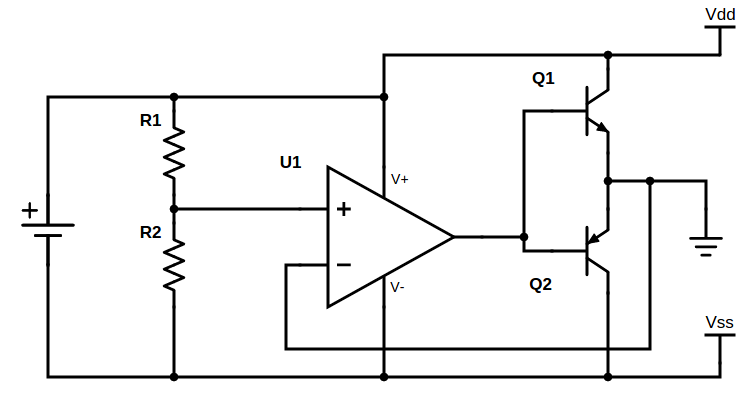
\includegraphics[scale=0.5]{img/fonte.png}
    \caption{Circuito para transformação de fonte assimétrica em simétrica com terra virtual.}
    \label{f_fonte}
\end{figure}

\subsection{Oscilador}
Para o amplificador U1 da figura \ref{f_sensor}, temos que 
\[
V_a = -\frac{\frac{1}{sC_1}}{R_1}V_b = -\frac{1}{sR_1C_1}Vb = -\frac{1}{R_1C_1} \int_{0}^{T}V_b(t)dt.
\]

Para $V_b(t) = cte.$, temos que 

\begin{equation}
V_a = -\frac{V_b}{R_1C_1}T.
\label{e_va}  
\end{equation}

No caso do amplificador U2,

\[
\frac{V_a - V_+}{R_2} = \frac{V_+ - V_b}{R_3} \quad \therefore \quad \frac{V_a}{R_2} - \frac{V_+}{R_2} = \frac{V_+}{R_3} - \frac{V_b}{R_3}
\]

e

\[
\frac{V_a}{R_2} + \frac{V_b}{R_3} = V_+ \bigg (\frac{1}{R_2} + \frac{1}{R_3} \bigg).
\]

Então, 

\[
    V_+ = \frac{V_aR_3 + V_bR_2}{R_3+R_2}.
\]


Assim, se $V_b = -V_{cc}$, $V_b$ irá para $+V_{cc}$ quando $V_+ = 0$, ou seja, quando $V_aR_3 = -V_bR_2$. Logo,

\[ V_a = -V_b\frac{R_2}{R_3} = +V_{cc}\frac{R_2}{R_3}. \]

Isso quer dizer que quando $V_a = +V_{cc}\frac{R_2}{R_3}$, $V_b$ passa de $-V_{cc}$ para $+V_{cc}$. De forma semelhante. pode ser demonstrado que, quando $V_a = -V_{cc}\frac{R_2}{R_3}$, $V_b$ passa de $+V_{cc}$ para $-V_{cc}$.

Portanto, definimos que, para o semiciclo positivo, temos

\begin{equation}
V_a = +V_{cc}\frac{R_2}{R_3},
\label{e_positivo}
\end{equation}

e para o semiciclo negativo

\begin{equation}
V_a = -V_{cc}\frac{R_2}{R_3}.
\label{e_negativo}
\end{equation}

Substituindo a equação \ref{e_va} em \ref{e_positivo},

\[
-\frac{-V_{cc}}{R_1C_1}T_1 = +V_{cc}\frac{R_2}{R_3}
\]

\[
    \therefore T_1 = \bigg ( \frac{R_2}{R_3}R_1\bigg )C_1
\]

e como $T = 4T_1$,

\begin{equation}
T =  4 \frac{R_2}{R_3} R_1C_1.
\label{e_periodo}
\end{equation}


\begin{figure}[H]
    \centering
    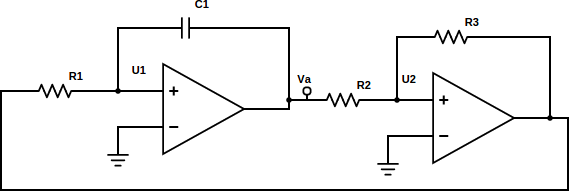
\includegraphics[scale=0.5]{img/sensor.png}
    \caption{Oscilador com amplificadores operacionais.}
    \label{f_sensor}
\end{figure} 


\newpage
\section{Metodologia Experimental}

\subsection{Materiais}
O material utilizado foi:

\begin{itemize}
	\item Protótipo do conversor Buck disponível no laboratório;
	\item CI 3524;
	\item AmpOp LM324;
	\item 2 potenciômetros de 10 $k \, \Omega$;
    \item 6 resistores de 1 $k \, \Omega$;
    \item 1 capacitor de 1 $nF$;
    \item 1 termistor de 10 $k \, \Omega$;
	\item Osciloscópio;
	\item Multímetro;
	\item Resistor variável de potência (50 $\Omega$).
\end{itemize}

Para execução do experimento, faz-se necessário executar os seguintes passos:

\begin{enumerate}
    \item montar o protótipo Buck (figura \ref{fig:buck}) com tensão de entrada de 30V.
	\item montar o circuito do controlador conforme a figura \ref{fig:sch}, alimentando o CI com 12V;
	\item ajustar o circuito para responder as perguntas da seção \ref{perguntas}.
\end{enumerate}

\begin{figure}[H]
    \centering
    \caption{Montagem do conversor Buck.}
    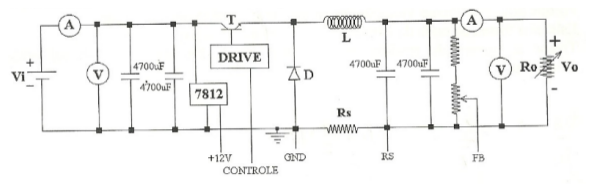
\includegraphics[scale=0.5]{buck}
    \label{fig:buck}
\end{figure}

\begin{figure}[H]
	\centering
	\caption{Controlador com CI SG3524.}
	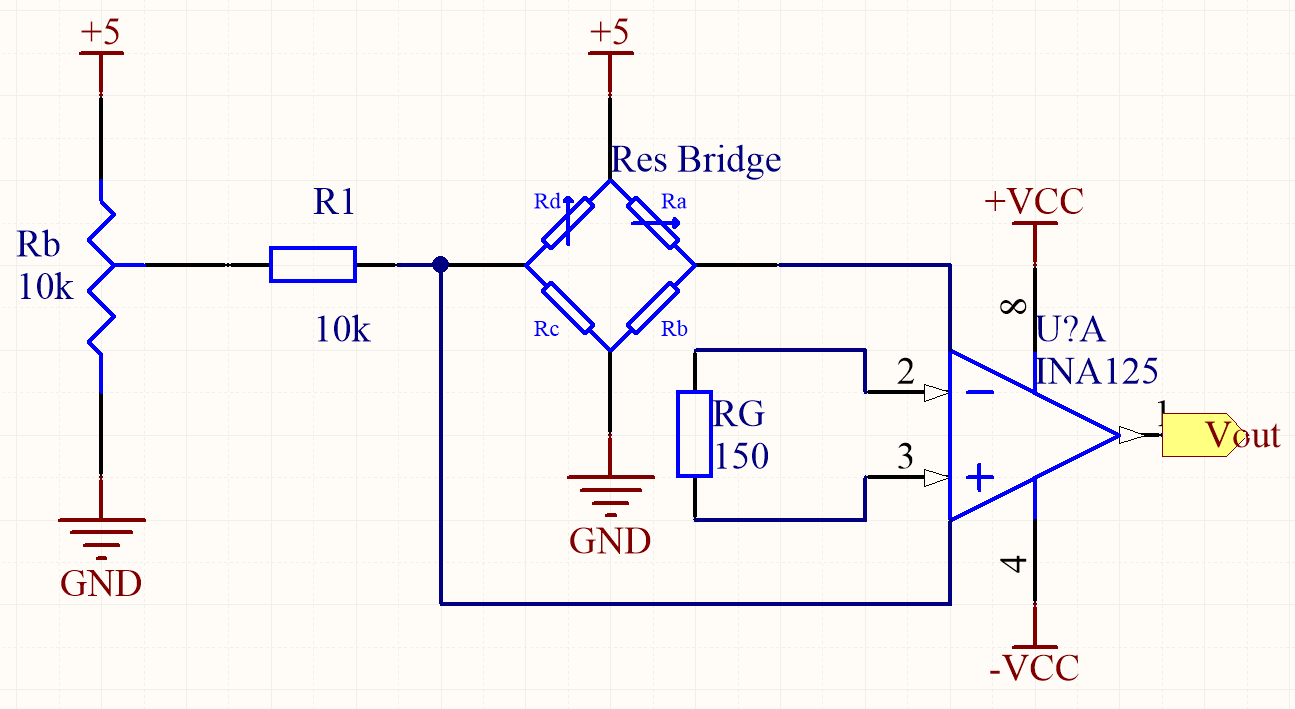
\includegraphics[scale=0.6]{sch}
	\label{fig:sch}
\end{figure}



\subsection{Questões}
\label{perguntas}

\begin{enumerate}
    \item Para ajustar a frequência dos pulsos de controle, utilizar um capacitor de 1 nF e potenciômetro de 10 $k \, \omega$; Variando o potenciômetro, ajuste a frequência de saída para 100 kHz com $K_c = 0.5$. Qual a frequência de saída se o $K_c$ for alterado para 1?
    
    \item Variando o potenciômetro, ajuste a frequência de saída para 50 kHz (ou um valor próximo a este) com $K_c = 0.5$. Qual é a frequência de saída se o $K_c$ for alterado para 1?
    
    \item Simular um aumento de temperatura utilizando um ferro de solda e o termistor NTC para cortar os pulsos de comando através do pino \textit{shutdown} do 3524;
    
    \item Para o controlador com $K_c = 0.5$ e frequência 100 kHz, qual a tensão de saída do conversor buck tendo como carga 25 $\omega$ / 1kW (ajustar o reostato para este valor)?
    
    \item Para o controlador com $K_c = 1$ e frequência 100 kHz, qual a tensão de saída do conversor buck tendo como carga 25 $\omega$ / 1kW (ajustar o reostato para este valor)?
    
    \item Quais os conversores que devem utilizar o $K_c = 0.5$? Cite três conversores.
    
    \item Quais os conversores que devem utilizar o $K_c = 1$? Cite três conversores.
    
\end{enumerate}
\newpage
\section{Resultados}

\subsection{Circuito de proteção com diodo Zener}
O diodo utilizado possui corrente máxima de $80mA$. Sendo assim, o valor de $R_z$ calculado, utilizando a equação \ref{e_rz}, foi de

\[ R_z = \frac{7.1 - 5.1}{80.10^{-3}} = 25 \Omega.\]

O valor comercial mais próximo, e que foi utilizado, é o de $27\Omega$.

A tabela \ref{t_zener} mostra os dados obtidos durante o experimento e a figura \ref{f_plotzener} mostra o gráfico.

\begin{small}
	\begin{table}[H]
		\begin{center}
			\caption{Tensão de entrada e tensão de saída para o diodo zener.}
			\begin{tabular}{l|l}
				\hline
				$V_{in}$ [V] & $V_o$ [V] \\
				\hline
				-2.02  & -0.840 \\
				\hline
				-1.40  & -0.822 \\
				\hline
				-0.8  & -0.757 \\
				\hline
				-0.2  & -0.220 \\
				\hline
				0.39  & 0.39 \\
				\hline
				1.00  & 1.00 \\
				\hline
				1.60  & 1.60 \\
				\hline
				2.25  & 2.24 \\
				\hline
				2.88  & 2.88 \\
				\hline
				3.37  & 3.37 \\
				\hline
				3.99  & 3.99 \\
				\hline
				4.64 & 4.64 \\
				\hline
				5.21 & 5.17 \\
				\hline
				5.81 & 5.26 \\
				\hline
				6.40 & 5.32 \\
				\hline
				6.98 & 5.37 \\
				\hline
			\end{tabular}
			\label{t_zener}
		\end{center}
	\end{table}
\end{small}


\begin{figure}[H]
	\centering
	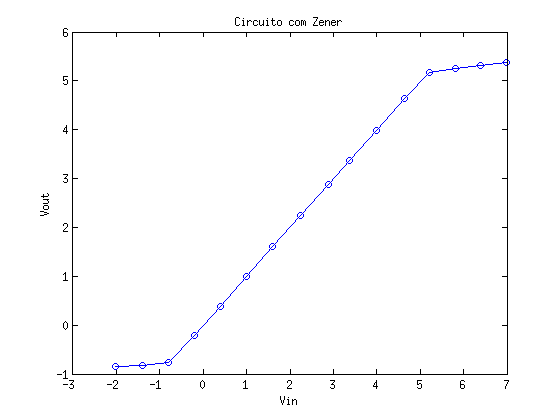
\includegraphics[scale=1]{img/plotzener.png}
	\caption{Circuito de proteção com diodo Zener.}
	\label{f_plotzener}
\end{figure}

\subsection{Circuito de proteção com diodo 1N4148}
O diodo utilizado possui corrente máxima de $200mA$. Sendo assim, o valor de $R_z$ calculado, utilizando a equação \ref{e_rz}, foi de

\[ R_z = \frac{7.1 - 5.1 - 0.7}{200.10^{-3}} = 6.5 \Omega.\]

O valor comercial mais próximo, e que foi utilizado, é o de $10\Omega$.

A tabela \ref{t_1n4148} mostra os dados obtidos durante o experimentoe a figura \ref{f_plot1n4148} mostra o gráfico.
\begin{small}
	\begin{table}[H]
		\begin{center}
			\caption{Tensão de entrada e tensão de saída para o diodo 1N4148.}
			\begin{tabular}{l|l}
				\hline
				$V_{in}$ [V] & $V_o$ [V] \\
				\hline
				0.00 & 0.00 \\
				\hline
				0.36 & 0.32 \\
				\hline
				0.90 & 0.81 \\
				\hline
				1.10 & 1.00 \\
				\hline
				1.60 & 1.45 \\
				\hline
				1.81 & 1.64 \\
				\hline
				2.03 & 1.86 \\
				\hline
				2.52 & 2.30 \\
				\hline
				2.95 & 2.70 \\
				\hline
				3.40 & 3.10 \\
				\hline
				3.85 & 3.53 \\
				\hline
				4.31 & 3.94 \\
				\hline
				4.77 & 4.33 \\
				\hline
				5.01 & 4.55 \\
				\hline
				5.46 & 4.95 \\
				\hline
			\end{tabular}
			\label{t_1n4148}
		\end{center}
	\end{table}
\end{small}

\begin{figure}[H]
	\centering
	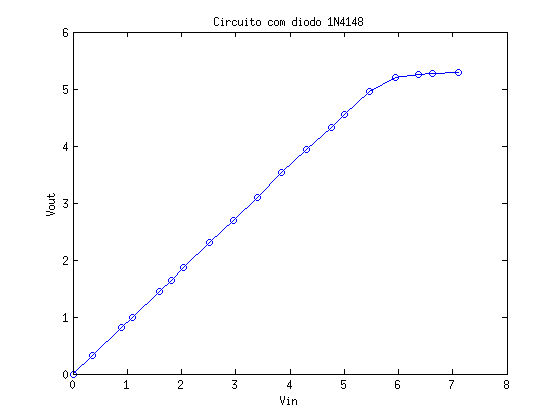
\includegraphics[scale=1]{img/plot1n4147.png}
	\caption{Circuito de proteção com diodo 1N4148.}
	\label{f_plot1n4148}
\end{figure}

\subsection{Circuito de proteção com diodo germânio}
O diodo utilizado possui corrente máxima de $1 \mu A$. Sendo assim, o valor de $R_z$ calculado, utilizando a equação \ref{e_rz}, foi de

\[ R_z = \frac{7.1 - 5.1 - 0.3}{1.10^{-6}} = 1.7 M \Omega.\]

O valor comercial mais próximo, e que foi utilizado, é o de $2 M \Omega$.

A tabela \ref{t_germânio} mostra os dados obtidos durante o experimento e a figura \ref{f_plotgermanio} mostra o gráfico.

\begin{small}
	\begin{table}[H]
		\begin{center}
			\caption{Tensão de entrada e tensão de saída para o diodo de germânio.}
			\begin{tabular}{l|l}
					\hline
					$V_{in}$ [V] & $V_o$ [V] \\
					\hline
					0.00 & 0.00 \\
					\hline
					0.40 & 0.40 \\
					\hline
					0.91 & 0.90 \\
					\hline
					1.51 & 1.50 \\
					\hline
					1.85 & 1.84 \\
					\hline
					2.17 & 2.17 \\
					\hline
					2.68 & 2.68 \\
					\hline
					3.06 & 3.06 \\
					\hline
					3.60 & 3.60 \\
					\hline
					3.96 & 3.96 \\
					\hline
					4.45 & 4.45 \\
					\hline
					4.96 & 4.96 \\
					\hline
					5.21 & 5.19 \\
					\hline
					5.92 & 5.27 \\
					\hline
					6.34 & 5.29 \\
					\hline
					6.79 & 5.29 \\
					\hline
					7.10 & 5.29 \\
					\hline
			\end{tabular}
			\label{t_germânio}
		\end{center}
	\end{table}
\end{small}

\begin{figure}[H]
	\centering
	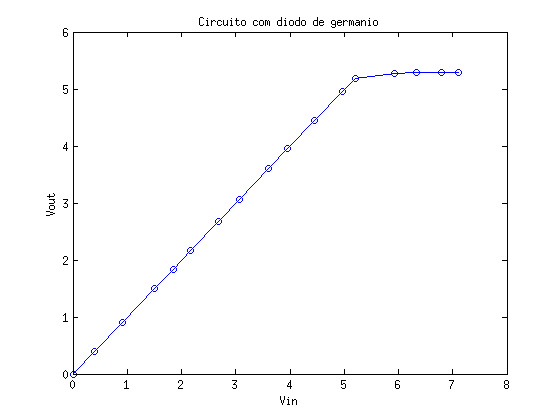
\includegraphics[scale=1]{img/plotgermanio.png}
	\caption{Circuito de proteção com diodo de germânio.}
	\label{f_plotgermanio}
\end{figure}

\subsection{Termistor com corrente constante}
A tabela \ref{t_termistor} mostra os dados obtidos para o termistor NTC com o circuito de corrente constante e a figura \ref{f_plottermistor} mostra a curva característica do sensor.

\begin{small}
	\begin{table}[H]
		\begin{center}
			\caption{Tensão de entrada e tensão de saída para o diodo de germânio.}
			\begin{tabular}{c|c}
				\hline
				$Temperatura$ [ºC] & $V_o$ [V] \\
				\hline
				26 & 7.35 \\
				\hline
				28 & 6.92 \\
				\hline
				29 & 6.81 \\
				\hline
				30 & 6.61 \\
				\hline
				31 & 6.63 \\
				\hline
				32 & 5.72 \\
				\hline
				33 & 6.32 \\
				\hline
				34 & 5.33 \\
				\hline
				35 & 5.47 \\
				\hline
				39 & 4.25 \\
				\hline
				42 & 3.85 \\
				\hline
				43 & 3.64 \\
				\hline
				46 & 3.33 \\
				\hline
				47 & 1.66 \\
				\hline
				52 & 1.35 \\
				\hline
				54 & 1.882 \\
				\hline
				56 & 1.19 \\
				\hline
				63 & 0.98 \\
				\hline
				68 & 0.93 \\
				\hline
				69 & 0.87 \\
				\hline
			\end{tabular}
			\label{t_termistor}
		\end{center}
	\end{table}
\end{small}

\begin{figure}[H]
	\centering
	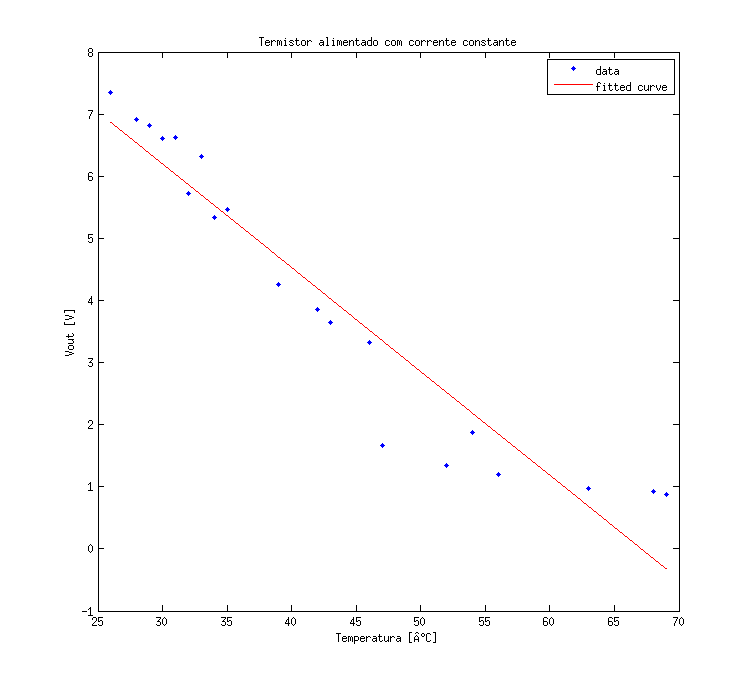
\includegraphics[scale=0.9]{img/plottermistor.png}
	\caption{Saída de tensão para o termistor NTC.}
	\label{f_plottermistor}
\end{figure}
\newpage
\section{Discussão e Conclusão}
Com base nos resultados obtidos, foi possível observar que o uso de diodos possibilita a proteção de circuitos contra surto de tensão. Notou-se que a tensão máxima de saída depende exclusivamente da queda de tensão no diodo utilizado, sendo os diodos zener os que proveem um melhor controle.
Os resistores $R_z$ e $R_1$ são utilizados de forma a limitar a corrente que passa pelos diodos, evitando a queima dos mesmos.

Para o experimento de condicionamento do termistor, foi visto que, para uma corrente constante, a tensão de saída do sistema varia de forma aproximadamente linear para a faixa de temperatura mensurada. Note que os dados obtidos possuem uma precisão ruim devido ao método utilizado para aumentar e amostrar a temperatura.
\newpage
\section{Referências}

[1] Roteiro da atividade prática.
\vspace{0.5cm}

[2] "Algum artigo". Altor, nome. Ano.
\vspace{0.5cm}


\end{document}